\begin{frame}
    \frametitle{Tipos de sensores}
    \footnotesize
    
    \begin{block}{Propioceptivos}
        Sensores propioceptivos miden valores internos del sistema (robot), por ejemplo, velocidad del motor, carga de la rueda, ángulos de articulación del brazo del robot y voltaje de la batería.
    \end{block}

    \begin{block}{Exteroceptivos}
        Sensores exteroceptivos adquieren información del entorno del robot, por ejemplo, medidas de distancia, intensidad de la luz y amplitud del sonido. Por lo tanto, el robot interpreta las mediciones de los sensores exteroceptivos para extraer características ambientales significativas.
    \end{block}

    \begin{block}{Pasivos}
        Los sensores pasivos miden la energía ambiental que ingresa al sensor. Los ejemplos de sensores pasivos incluyen sondas de temperatura, micrófonos y cámaras.
    \end{block}

    \note{Las tecnologías de las cámaras pueden ser CCD (Charge Coupled Device) o CMOS (Complementary Metal Oxide Semiconductor)}

    \begin{block}{Activos}
        Los sensores activos emiten energía al medio ambiente y luego miden la reacción ambiental. Debido a que los sensores activos pueden gestionar interacciones más controladas con el medio ambiente, a menudo logran un rendimiento superior. Sin embargo, la detección activa presenta varios riesgos: la energía de salida puede afectar a otros sensores. las mismas características que el sensor está intentando medir.
        
        \note{Además, un sensor activo puede sufrir interferencias entre su señal y las que están fuera de su control. Por ejemplo, las señales emitidas por otros robots cercanos, o sensores similares en el mismo robot, pueden influir en las mediciones resultantes. La energía de salida puede afectar a las mismas características que el sensor está intentando medir. Los ejemplos de sensores activos incluyen codificadores de cuadratura de rueda, sensores ultrasónicos y telémetros láser.}
    \end{block}


\end{frame}


\begin{frame}
    \frametitle{Sensores}
    \note{tabla 4.1 del libro siegwart}
   
    \centering
    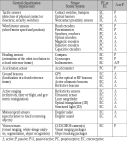
\includegraphics[height=0.9\textheight]{images/sensors_table.pdf} 

\end{frame}



\begin{frame}
    \frametitle{TODOs generales}
    \TODO{agregar a cada sensor una imagen de un sensor real}    
\end{frame}



